\section{Analysis techniques}
\label{sec:method} 
\mc{Ashley: I think somewhere in here (probably near the beginning) you need to describe how the 3 regions are combined, since I think you model their selection function separately and then combine for almost all results shown.}\mr{MR: I mention it the beginning of 2.1.2 and 4. Do you think it should mention it here?}


\subsection{Power spectrum estimator}
We first construct the density contrast field from the LRG density, $\rho$,
\begin{align}\label{eq:delta}
    \delta_{g} &= \frac{\rho- \overline{\rho}}{\overline{\rho}},
\end{align}
where the mean galaxy density $\overline{\rho}$ is estimated from the entire LRG sample. As a robustness test, we also analyze the power spectrum from each imaging region individually, in which $\overline{\rho}$ is calculated separately for each region. Then, we use the pseudo angular power spectrum estimator \citep{hivon2002master},
\begin{equation}\label{eq:pusedocell}
        \tilde{C}_{\ell} = \frac{1}{2\ell +1} \sum_{m=-\ell}^{\ell} |a_{\ell m}|^{2},
\end{equation}
where the coefficients $a_{\ell m}$ are obtained by decomposing $\delta_{g}$ into spherical harmonics, $Y_{\ell m}$,
\begin{equation}\label{eq:alm}
        a_{\ell m} = \int d\Omega ~ \delta_{g} W Y^{*}_{\ell m},
\end{equation}
where $W$ represents the survey window that is described by the number of randoms normalized to the expected value.

We use the implementation of \texttt{anafast} from the \textsc{HEALPix} package \citep{gorski2005healpix} to do fast harmonic transforms (Equation \ref{eq:alm}) and estimate the pseudo angular power spectrum of the LRG targets and the cross power spectrum between the LRG targets and the imaging systematic maps.

\subsection{Modelling}
The estimator in Equation \ref{eq:pusedocell} yields a biased power spectrum when the survey sky coverage is incomplete. Specifically, the survey mask causes correlations between different harmonic modes \citep{beutler2014clustering,wilson2017rapid}, and the measured clustering power is smoothed on scales near the survey size. An additional potential cause of systematic error arises from the fact that the mean galaxy density used to construct the density contrast field (Equation \ref{eq:delta}) is estimated from the available data, rather than being known a priori. This introduces what is known as an integral constraint effect, which can cause the power spectrum on modes near the size of the survey to be artificially suppressed, effectively pushing it towards zero \citep{peacock1991large,de2019integral}. Since the clustering power on these scales are highly sensitive to $\fnl$, it is crucial to account for these systematic effects in the model galaxy power spectrum to obtain unbiased $\fnl$ constraints \citep[see, also,][]{riquelme2022primordial}, which we describe below.
  
The other theoretical systematic issues are however subdominant in the angular power spectrum. For instance, relativistic effects generate PNG-like scale-dependent signatures on large scales, which interfere with measuring $\fnl$ with the scale-dependent bias effect using higher order multipoles of the 3D power spectrum \citep{wang2020}. Similarly, matter density fluctuations with wavelengths larger than survey size, known as super-sample modes, modulate the galaxy 3D power spectrum \citep{castorina2020JCAP}. In a similar way, the peculiar motion of the observer can mimic a PNG-like scale-dependent signature through aberration, magnification and the Kaiser-Rocket effect, i.e., a systematic dipolar apparent blue-shifting in the direction of the observer's peculiar motion \citep{2021JCAP...11..027B}.
  
\subsubsection{Angular power spectrum}
\mc{Santi: would nonlinear power spectrum matter? Somewhere here we should mention that the non-linear P(k) matter does not matter, maybe provide a reference.} The relationship between the linear matter power spectrum $P(k)$ and the projected angular power spectrum of galaxies is expressed by the following equation:
\begin{equation}\label{eq:cell}
C_{\ell} = \frac{2}{\pi}\int_{0}^{\infty}\frac{dk}{k}k^{3}P(k)|\Delta_{\ell}(k)|^{2} + N_{\rm shot},
\end{equation}
where $N_{\rm shot}$ is a scale-independent shot noise term. The projection kernel $\Delta_{\ell}(k) = \Delta^{\rm g}_{\ell}(k) + \Delta^{\rm RSD}_{\ell}(k)$ includes redshift space distortions and determines the contribution of each wavenumber $k$ to the galaxy power spectrum on mode $\ell$. For more details, refer to \cite{Padmanabhan2007}. The FFTLog\footnote{\href{https://github.com/xfangcosmo/FFTLog-and-beyond}{github.com/xfangcosmo/FFTLog-and-beyond}} algorithm and its extension as implemented in \cite{fang2020beyond} are employed to calculate the integrals for the projection kernel $\Delta_{\ell}(k)$, which includes the $l^{\rm th}$ order spherical Bessel functions, $ j_{\ell}(kr)$, and its second derivatives,
\begin{align}
    \Delta^{\rm g}_{\ell}(k) &= \int \frac{dr}{r} r (b+\Delta b) D(r) \frac{dN}{dr} j_{\ell}(kr),\\
    \Delta^{\rm RSD}_{\ell}(k) &= - \int \frac{dr}{r} r f(r) D(r) \frac{dN}{dr} j^{\prime\prime}_{\ell}(kr),
\end{align}
where $b$ is the linear bias (dashed curve in Figure \ref{fig:nz}), $D$ represents the linear growth factor normalized as $D(z=0)=1$, $f(r)$ is the growth rate, and $dN/dr$ is the redshift distribution of galaxies normalized to unity and described in terms of comoving distance\footnote{$dN/dr = (dN/dz)*(dz/dr) \propto (dN/dz)*H(z)$} (solid curve in Figure \ref{fig:nz}). The PNG-induced scale-dependent shift is given by \citep[see, also,][]{slosar2008constraints}
\begin{equation}
\Delta b = b_{\phi}(z) \fnl \frac{3 \Omega_{m} H^{2}_{0}}{2 k^{2}T(k)D(z) c^{2}} \frac{g(\infty)}{g(0)},
\label{eq:scaledepbias}
\end{equation}
where $\Omega_{m}$ is the matter density, $H_{0}$ is the Hubble constant\footnote{$H_{0}=100~({\rm km}~{\rm s}^{-1})/(h^{-1}{\rm Mpc})$ and $k$ is in unit of $h {\rm Mpc}^{-1}$}, $T(k)$ is the transfer function, and $g(\infty)/g(0) \sim 1.3$ with $g(z)\equiv (1+z) D(z)$ is the growth suppression due to non-zero $\Lambda$ because of our normalization of $D$ \citep[see, e.g.,][]{2010JCAP...07..013R, 2019MNRAS.485.4160M}. Assuming the universality relation, $b_{\phi} = 2 \delta_{c}(b - p)$, where $p=1$ and $\delta_{c}= 1.686$ is the critical density for spherical collapse \citep{fillmore1984self}. Provided that the uncertainty on $b_{\phi}$ only impacts the error on $\fnl$, and not the maximum likelihood estimate, we fix $p=1$ in our analysis for our sample of DESI LRG targets \citep[see, also,][]{slosar2008constraints,2010JCAP...07..013R,2013MNRAS.428.1116R}. We do not marginalize over $p$ to avoid parameter-space projection effects \citep{2022JCAP...11..013B}.

\begin{figure}
\centering
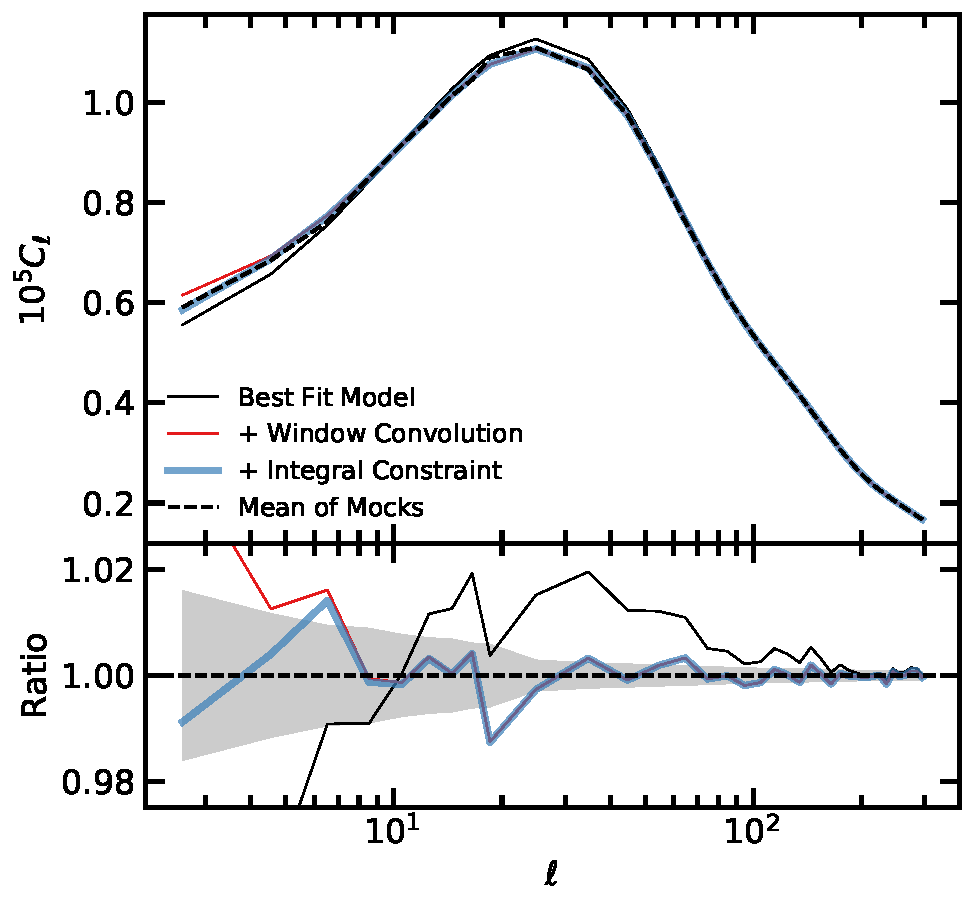
\includegraphics[width=0.45\textwidth]{model_mock.pdf}
\caption{The mean power spectrum from the $\fnl=0$ mocks (no contamination) and best-fitting theoretical prediction after accounting for the survey geometry and integral constraint effects. The dark and light shades represent the $68\%$ error on the mean and one realization, respectively. Bottom panel shows the residual power spectrum relative to the mean power spectrum. No imaging systematic cleaning is applied to these mocks.}\label{fig:model_mock}
\end{figure}



\subsubsection{Survey geometry and integral constraint}
We employ a technique similar to the one proposed by \cite{chon2004fast} to account for the impact of the survey geometry on the theoretical power spectrum. The ensemble average for the partial sky power spectrum is related to that of the full sky power spectrum via a mode-mode coupling matrix, ${\rm M}_{\ell \ell^{\prime}}$,
\begin{equation}\label{eq:mixm}
    <\tilde{C}_{\ell}> = \sum_{\ell^{\prime}} {\rm M}_{\ell \ell^{\prime}}<C_{\ell^{\prime}}>.
\end{equation}
We convert this convolution in the spherical harmonic space into a multiplication in the correlation function space. Specifically, we first transform the theory power spectrum (Equation \ref{eq:cell}) to the correlation function, $\hat{\omega}^{\rm model}$. Then, we estimate the survey mask correlation function, $\hat{\omega}^{\rm window}$, and obtain the pseudo-power spectrum,
\begin{align}
    \tilde{C}^{\rm model}_{\ell} &= 2\pi \int \hat{\omega}^{\rm model}\hat{\omega}^{\rm window}~P_{\ell}(\cos \theta) d\theta.
\end{align}

The integral constraint is another systematic effect which is induced since the mean galaxy density is estimated from the observed galaxy density, and therefore is biased by the limited sky coverage \citep{peacock1991large}. To account for the integral constraint, the survey mask power spectrum is used to introduce a scale-dependent correction factor that needs to be subtracted from the power spectrum as,
\begin{equation}
     \tilde{C}^{\rm model, IC}_{\ell} = \tilde{C}^{\rm model}_{\ell} - \tilde{C}^{\rm model}_{\ell=0} \left(\frac{\tilde{C}^{\rm window}_{\ell}}{\tilde{C}^{\rm window}_{\ell=0}}\right),
\end{equation}
where $\tilde{C}^{\rm window}$ is the survey mask power spectrum, i.e., the spherical harmonic transform of $\hat{\omega}^{\rm window}$.

The lognormal simulations are used to validate our survey window and integral constraint correction. Figure \ref{fig:model_mock} shows the mean power spectrum of the $\fnl=0$ simulations (dashed) and the best-fitting theory prediction before and after accounting for the survey mask and integral constraint. The simulations are neither contaminated nor mitigated. The light and dark shades represent the 68\% estimated error on the mean and one single realization, respectively. The DESI mask, which covers around $40\%$ of the sky, is applied to the simulations. We find that the survey window effect modulates the clustering power on $\ell < 200$ and the integral constraint alters the clustering power on $\ell < 6$.

\subsection{Parameter estimation}

Our parameter inference uses standard MCMC sampling. A constant clustering amplitude is assumed to determine the redshift evolution of the linear bias of our DESI LRG targets, $b(z) = b/D(z)$, which is supported by the HOD fits to the angular power spectrum \citep{zhou2021clustering}. In MCMC, we allow $\fnl$, $N_{\rm shot}$, and $b$ to vary, while all other cosmological parameters are fixed at the fiducial values (see \S \ref{ssec:mocks}). The galaxy power spectrum is divided into a discrete set of bandpower bins with $\Delta\ell=2$ between $\ell=2$ and $20$ and $\Delta \ell=10$ from $\ell=20$ to $300$. Each clustering mode is weighted by $2\ell+1$ when averaging over the modes in each bin.

The expected large-scale power is highly sensitive to the value of $\fnl$ such that the the amplitude of the covariance for $C_{\ell}$ is influenced by the true value of $\fnl$ \citep[see, e.g.,][for a discussion]{2013MNRAS.428.1116R}. As illustrated in the top row of Figure \ref{fig:histcell}, we find that the distribution of the power spectrum at the lowest bin, $2\leq \ell < 4$, is highly asymmetric and its standard deviation varies significantly from the simulations with $\fnl=0$ to $76.9$. We can make the covariance matrix less sensitive to $\fnl$ by taking the log transformation of the power spectrum, $\log C_{\ell}$. As shown in the bottom panels in Figure \ref{fig:histcell}, the log transformation reduces the asymmetry and the difference in the standard deviations between the $\fnl=0$ and $76.9$ simulations. Therefore, we minimize a negative likelihood defined as,
\begin{equation}
-2\ln\mathcal{L} = (\log \tilde{C}(\Theta)-\log \tilde{C})^{\dagger} \mathbb{C}^{-1} (\log \tilde{C}(\Theta)-\log \tilde{C}),
\end{equation}
where $\Theta$ represents a container for the parameters $\fnl$, $b$, and $N_{\rm shot}$; $\tilde{C}(\Theta)$ is the (binned) expected pseudo-power spectrum; $\tilde{C}$ is the (binned) measured pseudo-power spectrum; and $\mathbb{C}$ is the covariance on $\log\tilde{C}$ constructed from the $\fnl=0$ simulations. Flat priors are implemented for all parameters: $\fnl \in [-1000, 1000]$, $N_{\rm shot} \in [-0.001, 0.001]$, and $b \in [0, 5]$. \mc{Anna: Some readers might wonder if the covariance estimated from the lognormal mocks is accurate enough. Could you add maybe some lines justifying this?}

\begin{figure*}
\centering
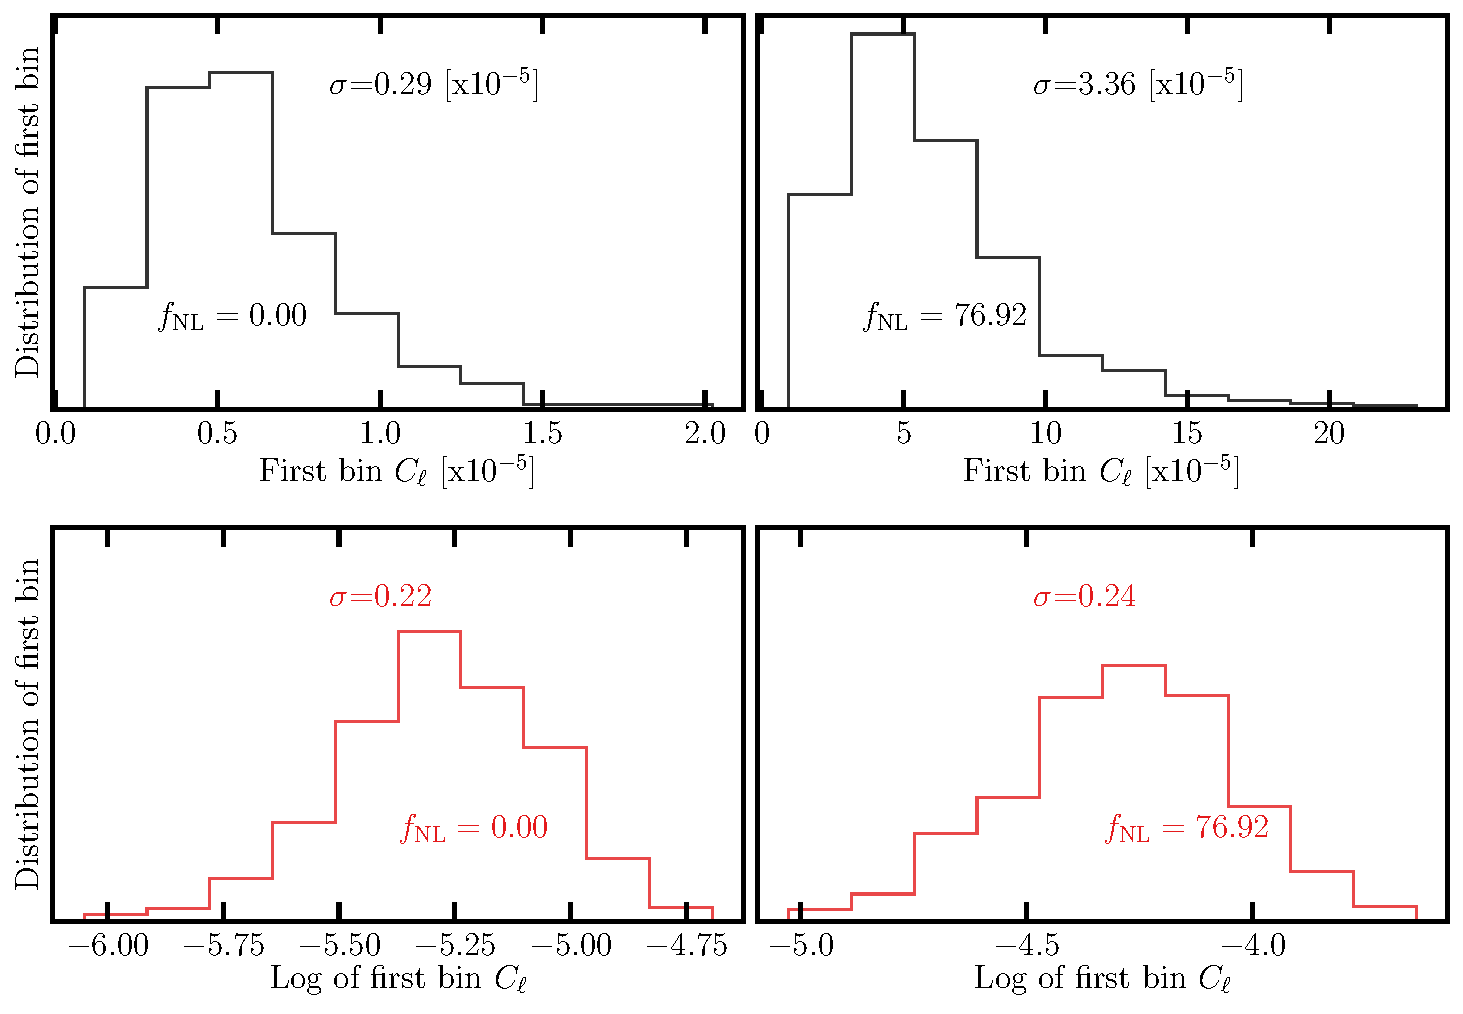
\includegraphics[width=0.85\textwidth]{hist_cl.pdf}
\caption{The distribution of the first bin power spectra and its log transformation from the simulations with $\fnl=0$ (left) and $76.92$ (right). The log transformation alleviates the asymmetry in the distributions.}\label{fig:histcell}
\end{figure*}




\subsection{Characterization of remaining systematics}
\label{ssec:characterization}
We briefly summarize two statistical tests based on the mean galaxy density contrast and the cross power spectrum between the galaxy density and the imaging systematic maps to assess the quality of the data and the significance of the remaining systematic effects \cite[see, also,][]{rezaie2021primordial}. We calculate these statistics and compare the values to those measured from the clean mocks before looking at the auto power spectrum of the DESI LRG targets.

\begin{figure*}
\centering
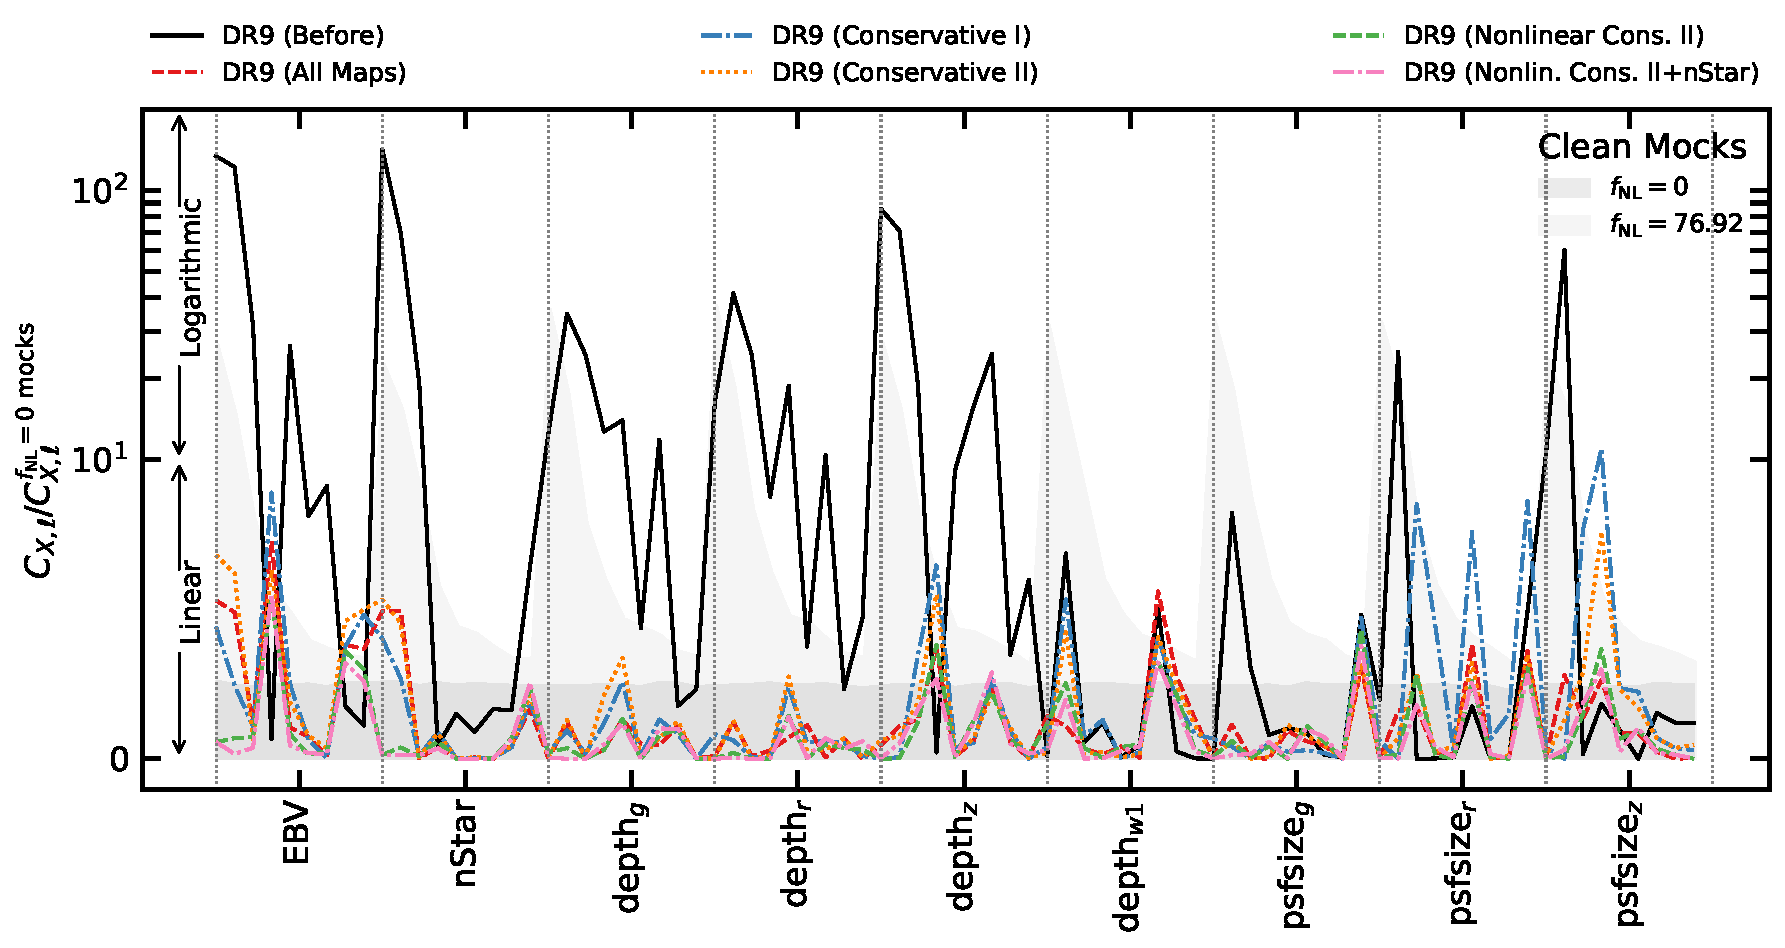
\includegraphics[width=0.95\textwidth]{clx_mocks.pdf}
\caption{The square of the cross power spectra between the DESI LRG targets and imaging systematic maps normalized by the auto power spectrum of the imaging systematic maps: Galactic extinction (EBV), stellar density (nStar), depth in \textit{grzw1} (depth$_{grzw1}$), and seeing in \textit{grz} (psfsize$_{grz}$). The black curves display the cross spectra before imaging systematic correction. The red, blue and orange curves represent the results after applying the imaging weights from the linear models trained with \textit{eight maps}, \textit{two maps}, and \textit{three maps}. The green and pink curves display the results after applying the imaging weights from the non-linear models trained with \textit{three maps} and \textit{four maps}. The dark and light shades represent the $97.5$ percentile from cross correlating the imaging systematic maps and the $\fnl=0$ and $76.9$ lognormal density fields, respectively.}\label{fig:clxmock}
\end{figure*}

\begin{figure*}
\centering
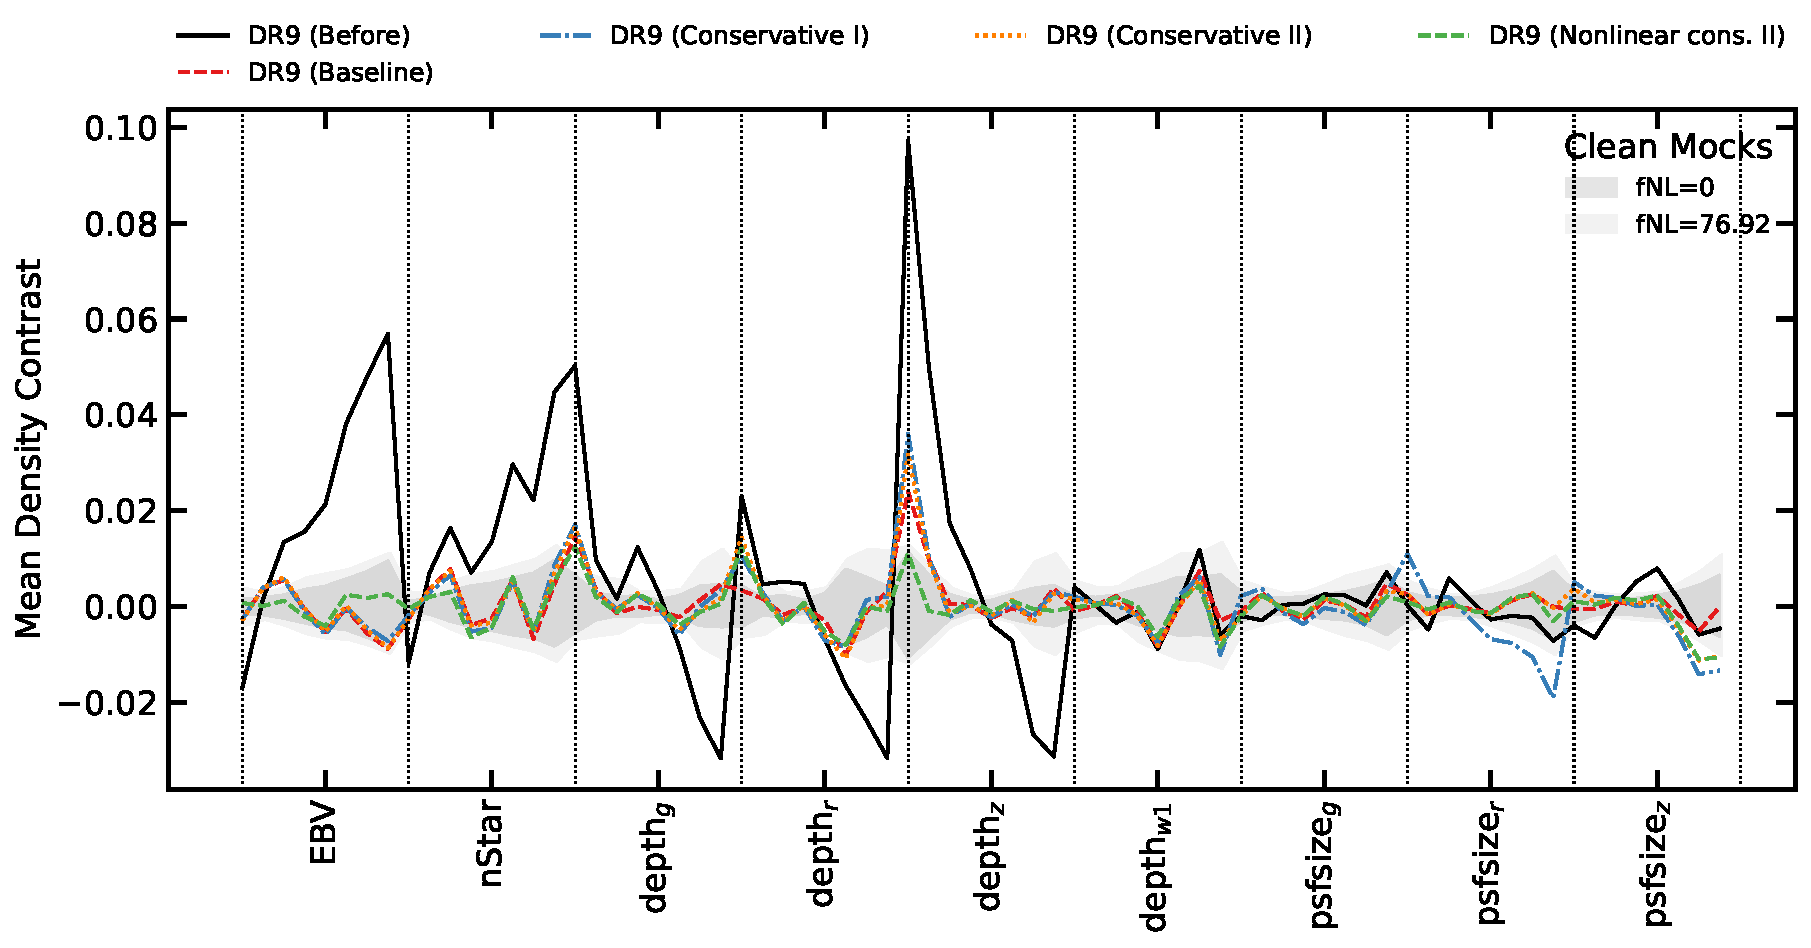
\includegraphics[width=0.95\textwidth]{nbar_mocks.pdf}
\caption{The mean density contrast of the DESI LRG targets as a function of the imaging systematic maps: Galactic extinction (EBV), stellar density (nStar), depth in \textit{grzw1} (depth$_{grzw1}$), and seeing in \textit{grz} (psfsize$_{grz}$). The black curves display the results before imaging systematic correction. The red, blue and orange curves represent the relationships after applying the imaging weights from the linear models trained with \textit{eight maps}, \textit{two maps}, and \textit{three maps}. The green and pink curves display the results after applying the imaging weights from the non-linear models trained with \textit{three maps} and \textit{four maps}. The dark and light shades represent the $68\%$ dispersion of 1000 lognormal mocks with $\fnl=0$ and $76.92$, respectively.}\label{fig:nbarmock}
\end{figure*}


\begin{figure}
\raggedleft
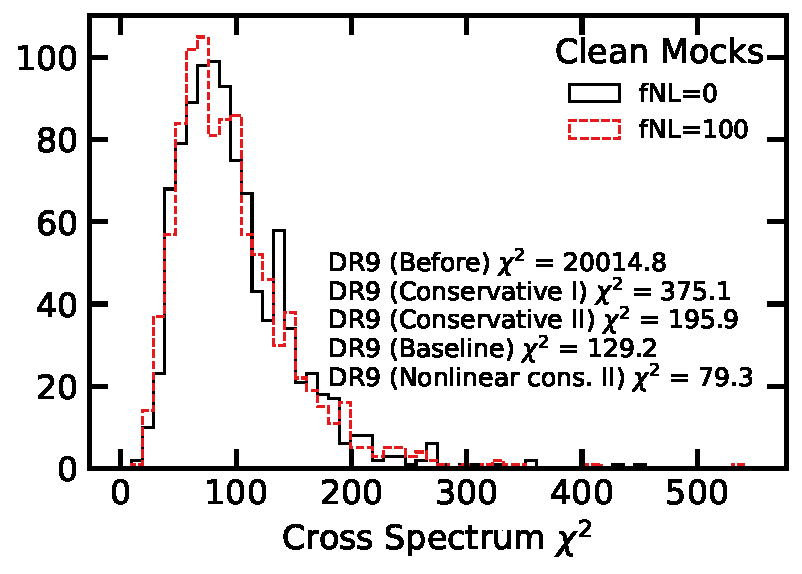
\includegraphics[width=0.45\textwidth]{chi2test.pdf}
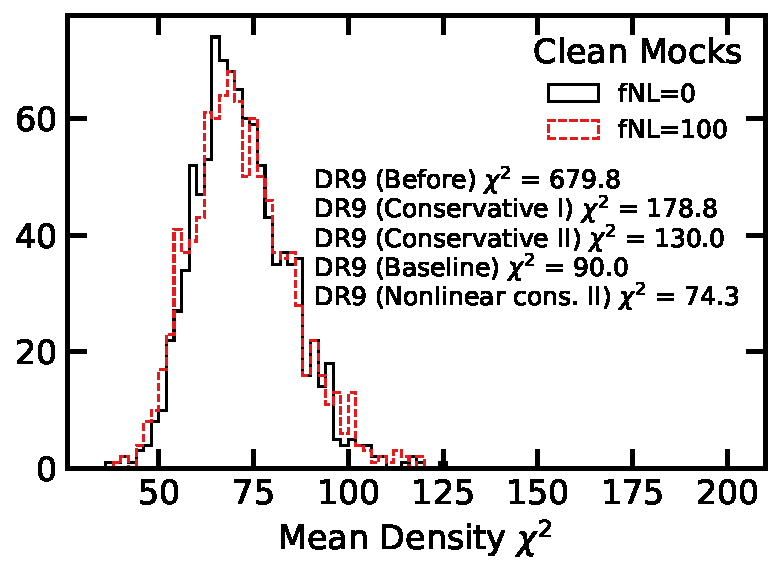
\includegraphics[width=0.44\textwidth]{chi2test2.pdf}
\caption{The remaining systematic error $\chi^{2}$ from the galaxy-imaging cross power spectrum (top) and the mean galaxy density contrast (bottom). The values observed in the DESI LRG targets before and after linear and non-linear treatments are quoted, and the histograms are constructed from 1000 realizations of clean lognormal mocks with $\fnl=0$ and $76.92$. \mc{Alex: can you show the DR9 chi2s as vertical lines rather than as text? Ashley: I think you could add one vertical dashed and/or dotted line to show the result for the Nonlinear 3 maps, which is what we adopt as the fiducial case.}}\label{fig:chi2test}
\end{figure}


\subsubsection{Cross power spectrum}

We characterize the cross correlations between the galaxy density and imaging systematic maps by
\begin{equation}
\tilde{C}_{X, \ell} = [\tilde{C}_{x_{1}, \ell}, \tilde{C}_{x_{2}, \ell}, \tilde{C}_{x_{3}, \ell}, ..., \tilde{C}_{x_{9}, \ell}],
\end{equation}
where $\tilde{C}_{x_{i}, \ell}$ represents the the square of the cross power spectrum between the galaxy density and $i^{\rm th}$ imaging map, $x_{i}$, divided by the auto power spectrum of $x_{i}$:
\begin{equation}
\tilde{C}_{x_{i}, \ell} = \frac{(\tilde{C}_{gx_{i}, \ell})^{2}}{\tilde{C}_{x_{i}x_{i},\ell}}.
\end{equation}
With this normalization, $\tilde{C}_{x_{i}}$ estimates the contribution of systematics up to the first order to the galaxy power spectrum. Then, the $\chi^{2}$ value for the cross power spectra is calculated via,
\begin{equation}
\chi^{2} = \tilde{C}^{T}_{X, \ell} \mathbb{C}_{X}^{-1} \tilde{C}_{X, \ell},
\end{equation}
where the covariance matrix $\mathbb{C}_{X} = < \tilde{C}_{X, \ell} \tilde{C}_{X, \ell'} >$ is constructed from the lognormal mocks. These $\chi^{2}$ values are measured for every clean mock realization with the \textit{leave-one-out} technique and compared to the values observed in the LRG sample with various imaging systematic corrections. Specifically, we use 999 realizations to estimate a covariance matrix and then apply the covariance matrix from the 999 realizations to measure the $\chi^{2}$ for the one remaining realization. This process is repeated for all 1000 realizations to construct a histogram for $\chi^{2}$. We only include the bandpower bins from $\ell=2$ to $20$ with $\Delta\ell=2$, and test for the robustness with higher $\ell$ modes in Appendix \ref{sec:scalesys}. 

Figure \ref{fig:clxmock} shows $\tilde{C}_{X}$ from the DESI LRG targets before and after applying various corrections for imaging systematics. The dark and light shades show the 97.5$^{\rm th}$ percentile from the $\fnl=0$ and $76.9$ mocks, respectively. Without imaging weights, the LRG sample has the highest cross-correlations against extinction, stellar density, and depth in z (solid black curve). There is less significant correlations against depth in the g and r bands, and psfsize in the z band, which could be driven because of the inner correlations between the imaging systematic maps. First, we consider cleaning the sample with the linear model using two maps (extinction and depth in r) as identified from the Pearson correlation. With linear two maps (dot-dashed blue curve), most of the cross power signals are reduced below statistical uncertainties, especially against extinction, stellar density, and depth. However, the cross power spectra against psfsize in r and z increases slightly on $6<\ell<20$ and $6<\ell<14$, respectively. Very likely, large-scale cross correlations ($\ell < 6$) are reduced using extinction and depth in the z-band, but there are some residual cross correlations on smaller scales ($\ell > 6$) which cannot be mitigated with our set of two maps. The linear three maps (dotted orange curve) approach alleviates the cross power spectrum against psfsize in r. On the other hand, non-linear three maps can reduce the cross correlations against both the r and z-band psfsize maps, which indicates the benefit of using a non-linear approach. For benchmark, we also show the normalized cross spectra after cleaning the LRG sample with linear eight maps and non-linear four maps. 

\subsubsection{Mean density contrast}
We calculate the histogram of the mean density contrast relative to the $j^{\rm th}$ imaging property, $x_{j}$:
\begin{equation}
\delta_{x_{j}} = ({\overline{\rho}})^{-1} \frac{\sum_{i} \rho_{i} W_{i}}{\sum_{i} W_{i}},
\end{equation}
where $\overline{\rho}$ is the global mean galaxy density, $W_{i}$ is the survey window in pixel $i$, and the summations over $i$ are evaluated from the pixels in every bin of $x_{j}$. We compute the histograms against all other imaging properties (see Figure \ref{fig:ng}). We use a set of eight equal-width bins for every imaging map, which results in a total of 72 bins. Then, we construct the total mean density contract as,
\begin{equation}
\delta_{X} = [\delta_{x_{1}}, \delta_{x_{2}}, \delta_{x_{3}}, ..., \delta_{x_{9}}],
\end{equation}
and the total residual error as,
\begin{equation}
\chi^{2} = \delta_{X}^{T} \mathbb{C_{\delta}}^{-1} \delta_{X},
\end{equation}
where the covariance matrix $\mathbb{C}_{\delta} = < \delta_{X} \delta_{X}>$ is constructed from the lognormal mocks. Figure \ref{fig:nbarmock} shows the mean density contrast against the imaging properties for the DESI LRG targets. The dark and light shades represent the $1\sigma$ level fluctuations observed in 1000 lognormal density fields respectively with $\fnl=0$ and $76.92$. The DESI LRG targets before treatment (solid curve) exhibits a strong trend around $10\%$ against the z-band depth which is consistent with the cross power spectrum. Additionally, there are significant spurious trends against extinction and stellar density at about $5-6\%$. The linear approach is able to mitigate most of the systematic fluctuations with only extinction and depth in the z-band as input; however,  a new trend appears against the r-band psfsize map with the \textit{linear two maps} approach (dot-dashed blue curve), which is indicative of the psfsize-related systematics in our sample. This finding is in agreement with the cross power spectrum. We re-train the linear model with three maps, but we still observe around $2\%$ residual spurious fluctuations in the low ends of depth and psfsize, in the z band, which implies non-linear systematic effects exist. We find that the imaging weights from the non-linear model trained with the three identified maps (or four maps including the stellar density) is capable of reducing the fluctuations below $2\%$. Even with the non-linear three maps, we have about $1\%$ remaining systematic fluctuations against the z-band psfsize. 


We use the $\chi^{2}$ statistics to assess how significant these fluctuations are in comparison to the clean mocks. Table \ref{tab:chi2test} summarizes the $\chi^{2}$ values observed in the data and the corresponding p-values inferred from the comparison to the clean $\fnl=0$ mocks. Figure \ref{fig:chi2test} shows the $\chi^{2}$ histograms from the normalized cross spectrum (top) and mean density contrast (bottom) statistics which are obtained from the $\fnl=0$ and $76.9$ lognormal mocks, respectively with dashed and solid lines. No mitigation is applied to these mocks, and thus the $\chi^{2}$ values are expected to be unbiased. The $\chi^{2}$ values observed in the DESI LRG targets are quoted for comparison, and the significance for each measurement is characterized by \textit{p-value} with respect to the $\fnl=0$ mocks without any mitigation applied to them. Before cleaning, our LRG sample has a cross power spectrum $\chi^{2}$ error of $20014.8$. After correction with the linear two maps approach, the cross spectrum $\chi^{2}$ is reduced to $375.1$ with p-value $=0.002$. Adding the r-band psfsize, the linear model reduces the $\chi^{2}$ down to $195.9$ with p-value $=0.044$; however, we can reject the null hypothesis that our sample with the linear three maps is properly cleaned at $95\%$ confidence. Even though cleaning with linear all maps gives the lowest cross spectrum $\chi^{2}$ of $129.2$ (and p-value $=0.239$), it potentially makes the analysis more prone to regressing out the true clustering signal, given the inner correlations among the imaging properties (Figure \ref{fig:pcc}). As an alternative, we apply the imaging weights from the non-linear method with the extinction, z-band depth, and r-band psfsize maps (\textit{non-linear three maps}). The cross power spectrum $\chi^{2}$ is reduced to $79.3$ with p-value $=0.594$. Adding the stellar density map reduces the cross power spectrum $\chi^{2}$ error to $70.9$ (p-value $=0.687$). Our cross power spectrum diagnostic supports the idea that a non-linear cleaning approach is needed to properly regress out the remaining spurious fluctuations. We investigate the test with the cross power spectrum up to higher multipoles but find no evidence of remaining systematic errors (see Appendix \ref{sec:scalesys}). 

\mc{Ashley: Add something at the end to clarify the reason that the extinction map can cause the stellar density trend is that they are strongly correlated.} Figure \ref{fig:chi2test} (bottom) shows the mean density $\chi^{2}$ observed in the mocks with or without $\fnl$. We find consistent results regardless of the underlying $\fnl$, which supports that our diagnostic is not sensitive to the fiducial cosmology. The values measured in the DESI LRG targets before and after applying imaging weights are quoted for comparison. The \textit{linear two maps} weights reduce the $\chi^{2}$ value from $679.8$ (before correction) to $178.8$. The p-value $=0$ indicates severe remaining systematic effects. Adding the r-band psfsize does not reduce the remaining systematics enough (p-value $=0$) even though the cleaning method yields a lower $\chi^{2}=130$. Training the linear model with all imaging systematic maps returns a more reasonable $\chi^{2}=90$ and p-value of $0.084$. However, regression with all imaging systematic maps as input can lead to the removal of the true clustering signal. With the imaging weights from the \textit{non-linear three maps} approach, we obtain a $\chi^{2}$ value of $74.3$ with p-value $=0.392$. Re-training the non-linear approach while adding the stellar density map (\textit{non-linear four maps}) yields minor improvement: $\chi^{2}=73.2$ and p-value $=0.422$. The minor impact on $\chi^{2}$ indicates that the stellar density trend in the mean LRG density can be explained via extinction since these two properties are strongly correlated; In regions with high stellar density, there is likely to be a higher concentration of dust, which can cause greater extinction of light.

\mc{Ashley: I would maybe add a new subsubsection (but at least a new paragraph) to summarize the results of the subsection, as they are quite important. This is also where I would discuss the tests that were done prior to looking at the data Cell. The discussion would basically provide a strong justification for the 3 map case being the fiducial case and point out that this was decided prior to seeing the data results. (Some of the words you wrote at the beginning of section 3.5 would go instead in this summary.)} The mean density contrast and cross power spectrum tests presented here show the effectiveness of the different cleaning approaches for the LRG sample before measuring the galaxy power spectrum and $\fnl$. As summarized in Table \ref{tab:chi2test}, the results of these tests reveal that cleaning the LRG sample with non-linear three maps produces statistically consistent $\chi^{2}$ values with the clean mocks. Based on these findings, we identify non-linear three maps as the optimal cleaning approach for the LRG sample, because adding more imaging systematics maps could potentially further complicate the over-correction issue.

\begin{table}
  \caption{Mean density and cross power spectrum $\chi^{2}$ and p-values that are inferred from the comparison to the $\fnl=0$ clean mocks.}\label{tab:chi2test}
  \begin{tabular}{lcccc}
    \hline
    \hline
    \multirow{2}{*}{\textbf{Cleaning Method}} &
      \multicolumn{2}{c}{\textbf{Mean Density}} &
      \multicolumn{2}{c}{\textbf{Cross Power Spectrum}} \\
    & $\chi^{2}$ & p-value & $\chi^{2}$ & p-value \\
    \hline
   No Weight & 679.8 & 0 & 20014.8 & 0 \\
   Linear Two Maps & 178.8 & 0 & 375.1 & 0\\
   Linear Three Maps & 130 & 0 & 195.9 & 0.04\\
   Linear Eight Maps & 90 & 0.08 & 129.2 & 0.24\\
   Non-linear Three Maps & 74.3 & 0.39  & 79.3 & 0.59\\
   Non-linear Four Maps & 73.2 & 0.42 & 70.9 & 0.69\\    
    \hline
  \end{tabular}
\end{table}


\subsection{Calibration of mitigation bias}\label{ssec:calibration}

\mc{Santi: How all of this was computed did not seem very clear to me. It seems that this part is what later determines that fnl!=0 from the data. So I think it would be worth explaining it more.} \mc{Ashley: I would find a way to *strongly* emphasize that the result does not depend at all on how the mocks were contaminated. Perhaps just a concluding sentence or two in its own paragraph along the lines} \mc{Ashley: It is important to note that we find nearly identical results for the mitigation bias whether or not the mocks have any contamination. This can be seen by observing the solid and dashed curves displayed on Fig. 9} The template-based mitigation of imaging systematics removes some of the true clustering signal, and the amount of the removed signal increases as more maps are used for the regression. We calibrate the over-correction effect using the mocks presented in \S \ref{sec:data}. We applied the neural network model to both the $\fnl=0$ and $76.9$ simulations, with and without imaging systematics, using various sets of imaging systematic maps. Specifically, we consider \textit{non-linear three maps}, \textit{non-linear four maps}, and \textit{non-linear nine maps}. Then, we measure the power spectra from the mocks. We fit both the mean power spectrum and each individual power spectrum from the mocks. Figure \ref{fig:fnlbias} displays a comparison between the estimates of $\fnl$ before and after mitigation for the clean mocks. The best-fitting estimates are represented by the solid curves, and the individual spectra results are displayed as the scatter points. The results from fitting the mean power spectrum of the contaminated mocks are also shown via the dashed curves. We find nearly identical results for the biases caused by mitigation, whether or not the mocks have any contamination, which can be seen by observing the solid and dashed curves displayed on Figure \ref{fig:fnlbias} (see, also, Figure \ref{fig:clmocks}, for a comparison of the mean power spectrum). For clarity, the best-fitting estimates for the individual contaminated data are not shown in the figure.

To calibrate our methods, we fit a linear curve to the $\fnl$ estimates from the mean power spectrum of the mocks, $f_{\rm NL, no~mitigation, clean} = m_{1} f_{\rm NL, mitigated} + m_{2}$. The $m_{1}$ and $m_{2}$ coefficients for non-linear three, four, and nine maps are summarized in Table \ref{tab:debiasparams}. These coefficients represent the impact of the cleaning methods on the likelihood. We find that the uncertainty in $\fnl$ after mitigation increases by $m_{1}-1$. Figure \ref{fig:fnlbias} also shows that the choice of our cleaning method can have significant implications for the accuracy of the measured $\fnl$, and careful consideration should be given to the selection of the primary imaging systematic maps and the calibration of the cleaning algorithms in order to minimize systematic uncertainties.

\begin{figure}
\centering
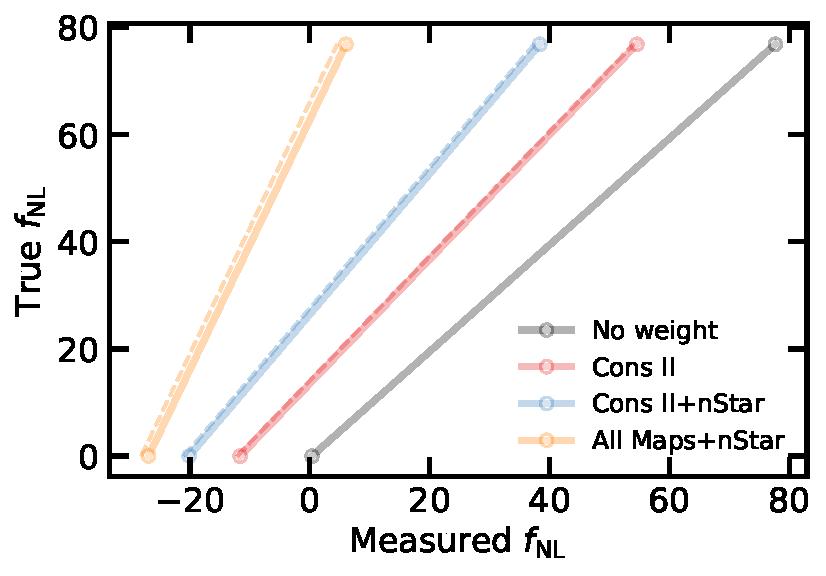
\includegraphics[width=0.45\textwidth]{figures/fnlbias}
\caption{The \textit{No mitigated, clean} vs \textit{mitigated} $\fnl$ values from the $\fnl=0$ and $76.9$ mocks. The solid (dashed) lines represent the best-fitting estimates from fitting the mean power spectrum of the clean (contaminated) mocks. The scatter points show the best-fitting estimates from fitting the individual spectra for the clean mocks.}\label{fig:fnlbias}
\end{figure}

\begin{table}
\begin{center}
\caption{Linear parameters employed to de-bias the $\fnl$ constraints to account for the over-correction issue. \mc{Ashley: You could also add the m1/m2 to the table for the clean mock case?}}\label{tab:debiasparams}
\begin{tabular}{lcc}
\hline
\hline
\textbf{Cleaning Method} & $m_{1}$ & $m_{2}$ \\
\hline
Non-linear Three Maps & 1.17 & 13.95 \\
Non-linear Four Maps & 1.32 & 26.97 \\
Non-linear Nine Maps & 2.35 & 63.5\\
\hline
\end{tabular}
\end{center}
\end{table}